\documentclass{article}
\usepackage{graphicx} % Required for inserting images
\graphicspath{ {./images/} }
\usepackage[usenames, dvipsnames, svgnames, table, x11names]{xcolor}
\usepackage{amsmath, amssymb, amsthm, amsfonts, mathtools, thmtools, bm}
\usepackage[framemethod=TikZ]{mdframed}
\usepackage{tcolorbox}
\usepackage{csquotes}
\tcbuselibrary{skins, breakable}
\usepackage[margin=1in]{geometry}
\usepackage{tikz}
\usepackage[super,square]{natbib}
\usepackage{eso-pic}

\newlength{\PageFrameTopMargin}
\newlength{\PageFrameBottomMargin}
\newlength{\PageFrameLeftMargin}
\newlength{\PageFrameRightMargin}

\setlength{\PageFrameTopMargin}{1cm}
\setlength{\PageFrameBottomMargin}{1cm}
\setlength{\PageFrameLeftMargin}{1cm}
\setlength{\PageFrameRightMargin}{1cm}

\makeatletter

\newlength{\Page@FrameHeight}
\newlength{\Page@FrameWidth}

\AddToShipoutPicture{
  \thinlines
  \setlength{\Page@FrameHeight}{\paperheight-\PageFrameTopMargin-\PageFrameBottomMargin}
  \setlength{\Page@FrameWidth}{\paperwidth-\PageFrameLeftMargin-\PageFrameRightMargin}
  \put(\strip@pt\PageFrameLeftMargin,\strip@pt\PageFrameTopMargin){
    \framebox(\strip@pt\Page@FrameWidth, \strip@pt\Page@FrameHeight){}}}

\makeatother
\begin{document}
\begin{center}
% Upper part of the page

\includegraphics[width=0.60\textwidth]{IISER-K_Logo.svg.png}\\[1cm]
\textsc{\LARGE}\\[1cm]
% Title

\centerline{\rule{1\linewidth}{.2pt}}
{ \huge \bfseries LS1202 Ecology Project: \\ Studying Flower Morphology of Various Species on Campus, at IISER Kolkata}
\centerline{\rule{1\linewidth}{.2pt}}


% Author
\Large
\emph{Authors:}\\
Abhratanu Ray - 22MS052\\
Aritra Barua - 22MS058\\
Swarnava Dam - 22MS053\\
Rishab P. Hariharan -22MS045\\
Manish Kumar - 22MS054\\
Sabarno Saha - 22MS037\\
\vfill
% Bottom of the page
{\Large Date : June 21, 2023}
\end{center}
\newpage

\title{LS1202 Project: Studying Flower Morphology of Various Species on Campus, at IISER Kolkata}
\author{Abhratanu Ray (22MS052), Rishab P. Hariharan (22MS045), Sabarno Saha (22MS037),}
\date{ Swarnava Dam (22MS053), Manish Kumar (22MS054), Aritra Barua (22MS058)}
%\date{June 2023}



%\maketitle

\section*{Introduction}
Throughout this project, we will share our observations on 5 different flower species, in our campus. We shall speak about their physical features, morphology and also of the interactions between them and their environment.

\section{Helianthus annus}
\begin{center}
    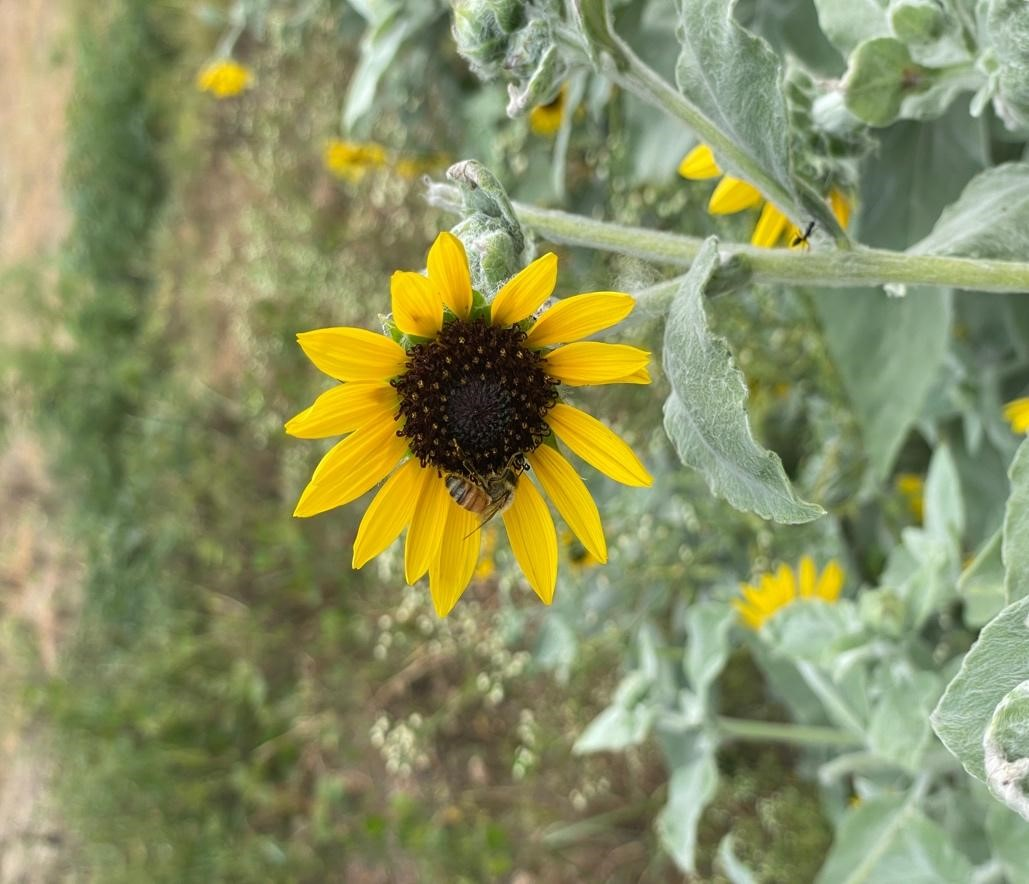
\includegraphics[scale=0.2]{images/1.jpg}
\end{center}
\textbf{Scientific name:} Helianthus annus\newline
\textbf{Common name:} Sunflower\newline
\textbf{Family:} Asteraceae\newline
\textbf{Location:} Near ICVS hostel\newline
\textbf{Flower:} Bisexual flower, each sunflower is actually an inflorescence with a large head (capitulum) that contains many tiny flowers called florets. There are two types of florets i.e., ray florets (zygomorphic) and disk florets (actinomorphic). \newline
\textbf{Pollination:} Entomophilous (pollinating agents are insects), a honeybee can be seen on the sunflower in the image.

% \newline
\text{ }\newline
\textbf{Ray Floret:} Unisexual, pistillate or neuter, zygomorphic, sessile, incomplete and sterile.\newline
\textbf{Calyx:} Reduced calyx (modified into pappus or absent or scale-like).\newline
\textbf{Corolla:}  Three petals are joined to form a strap, and in the case of 5 petals, they form a ligule, valvate, highly coloured.\newline
\textbf{Androecium:} Absent\newline
\textbf{Gynoecium:} Either absent or if present then bicarpellary, syncarpous, inferior, unilocular with basal placentation, one anatropous ovule; style one; stigma bifid.
\begin{center}
    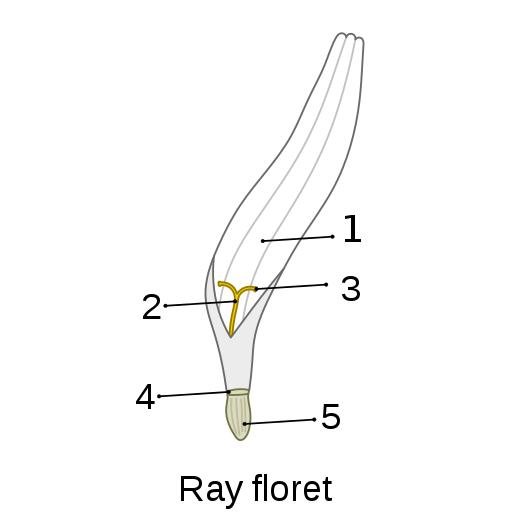
\includegraphics[scale=0.45]{images/2.png}
\end{center}

\text{ }\newline
\textbf{Disk Floret}: Bisexual, complete, actinomorphic and sessile (no pedicle)
\begin{center}
    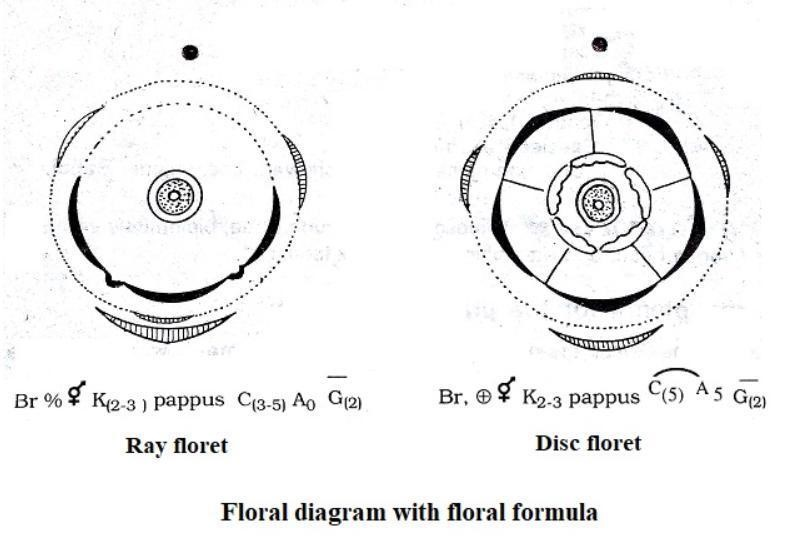
\includegraphics[scale=0.5]{images/3.jpg}
\end{center}
% \newline
\text{ }\newline
\textbf{Calyx:} modified into pappus or scale, persistent.
Corolla: petals 5, gamopetalous, tubular, valvate and coloured.\newline

\textbf{Androecium:} 5 stamen, epipetalous.\newline
\textbf{Gynoecium:} Bicarpellary, syncarpous, epigynous ovary (inferior), unilocular with single anatropous ovule, basal placentation; style simple, long, stigma bifid.
\section{Nerium oleander}
\begin{center}
    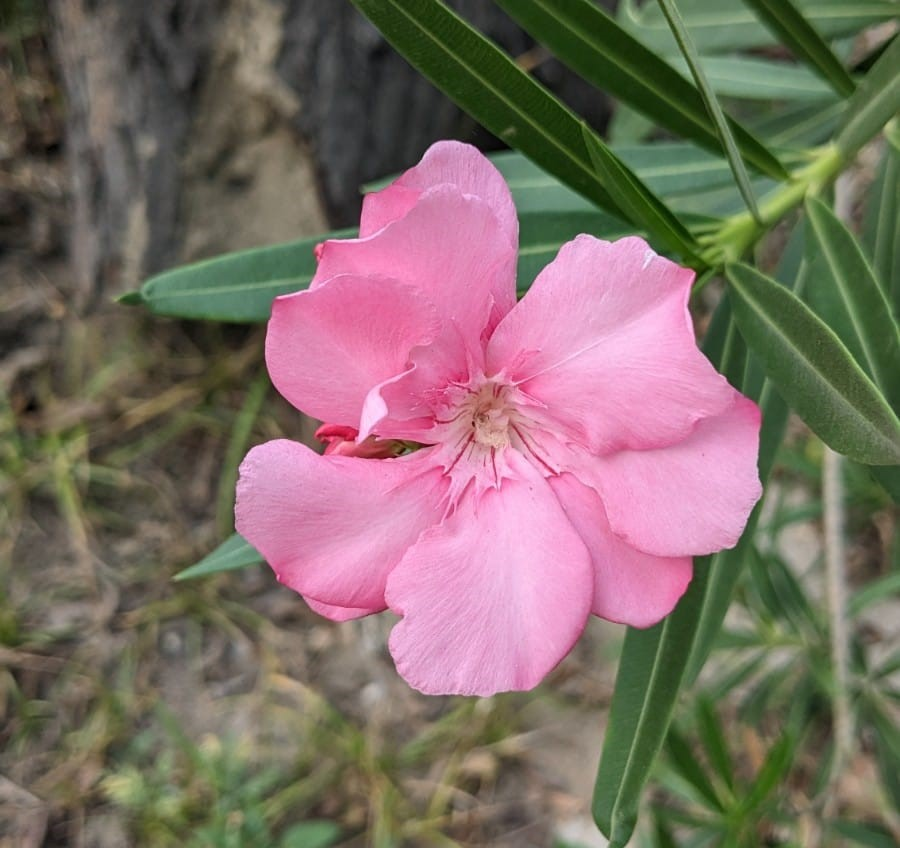
\includegraphics[scale=0.3]{images/WhatsApp Image 2023-06-19 at 13.52.19.jpg}
\end{center}
\textbf{Scientific name:} Nerium oleander\newline
\textbf{Common name:} Oleander\newline
\textbf{Family:} Apocynaceae\newline
\textbf{Location:} Near ICVS hostel\newline
\textbf{Flower:} Bisexual flower, Nerium oleander flowers are borne in terminal clusters known as cymes. Each cyme consists of several individual flowers that arise from a common point. The flowers of Nerium oleander are large and showy, with a funnel-shaped or salverform (tube-like) structure. They typically measure around 4-5 cm (1.5-2 inches) in diameter.  \newline
\textbf{Pollination:} Oleanders conduct \enquote{deceit} pollination. They lure pollinators in with a sweet smell and showy flowers, but there is no nectar to be found. Pollinators burn precious energy while pollinating oleanders, with no reward for their work.

\text{ }\newline
\textbf{Calyx:} The calyx has 5 unfused, green sepals.\newline
\textbf{Corolla:} The corolla has 5 red, white, or pink petals that are fused forming a tube with the lobes overlapping to one side forming a pinwheel shape.\newline
\textbf{Androecium:} It consists of five stamens alternating with
the petals. The stamens are situated on the tube or the
throat of the corolla (i.e., epipetalous). The filaments are
short, anthers introrse, polyandrous or connate and often
adhere to the stigma. The anther lobes are sometimes
empty at their base and prolonged into spines\newline
\textbf{Gynoecium:} It consists of two carpels. The carpels may be
free (apocarpous) or connate (syncarpous); superior,
sometimes partly inferior as in Plumeria. The style is
simple and the stigma is thick and often bilobed. Rarely
the number of carpels exceeds, i.e., 3 to 5. Usually a
nectar secreting disc is situated beneath the gynoecium.
In syncarpous gynoecium, the ovary may be unilocular
with parietal placentation or marginal.
\begin{center}
    
\includegraphics{images/Screenshot 2023-06-21 235234.png}
\end{center}
\section{Plumeria pudica}
\begin{center}
    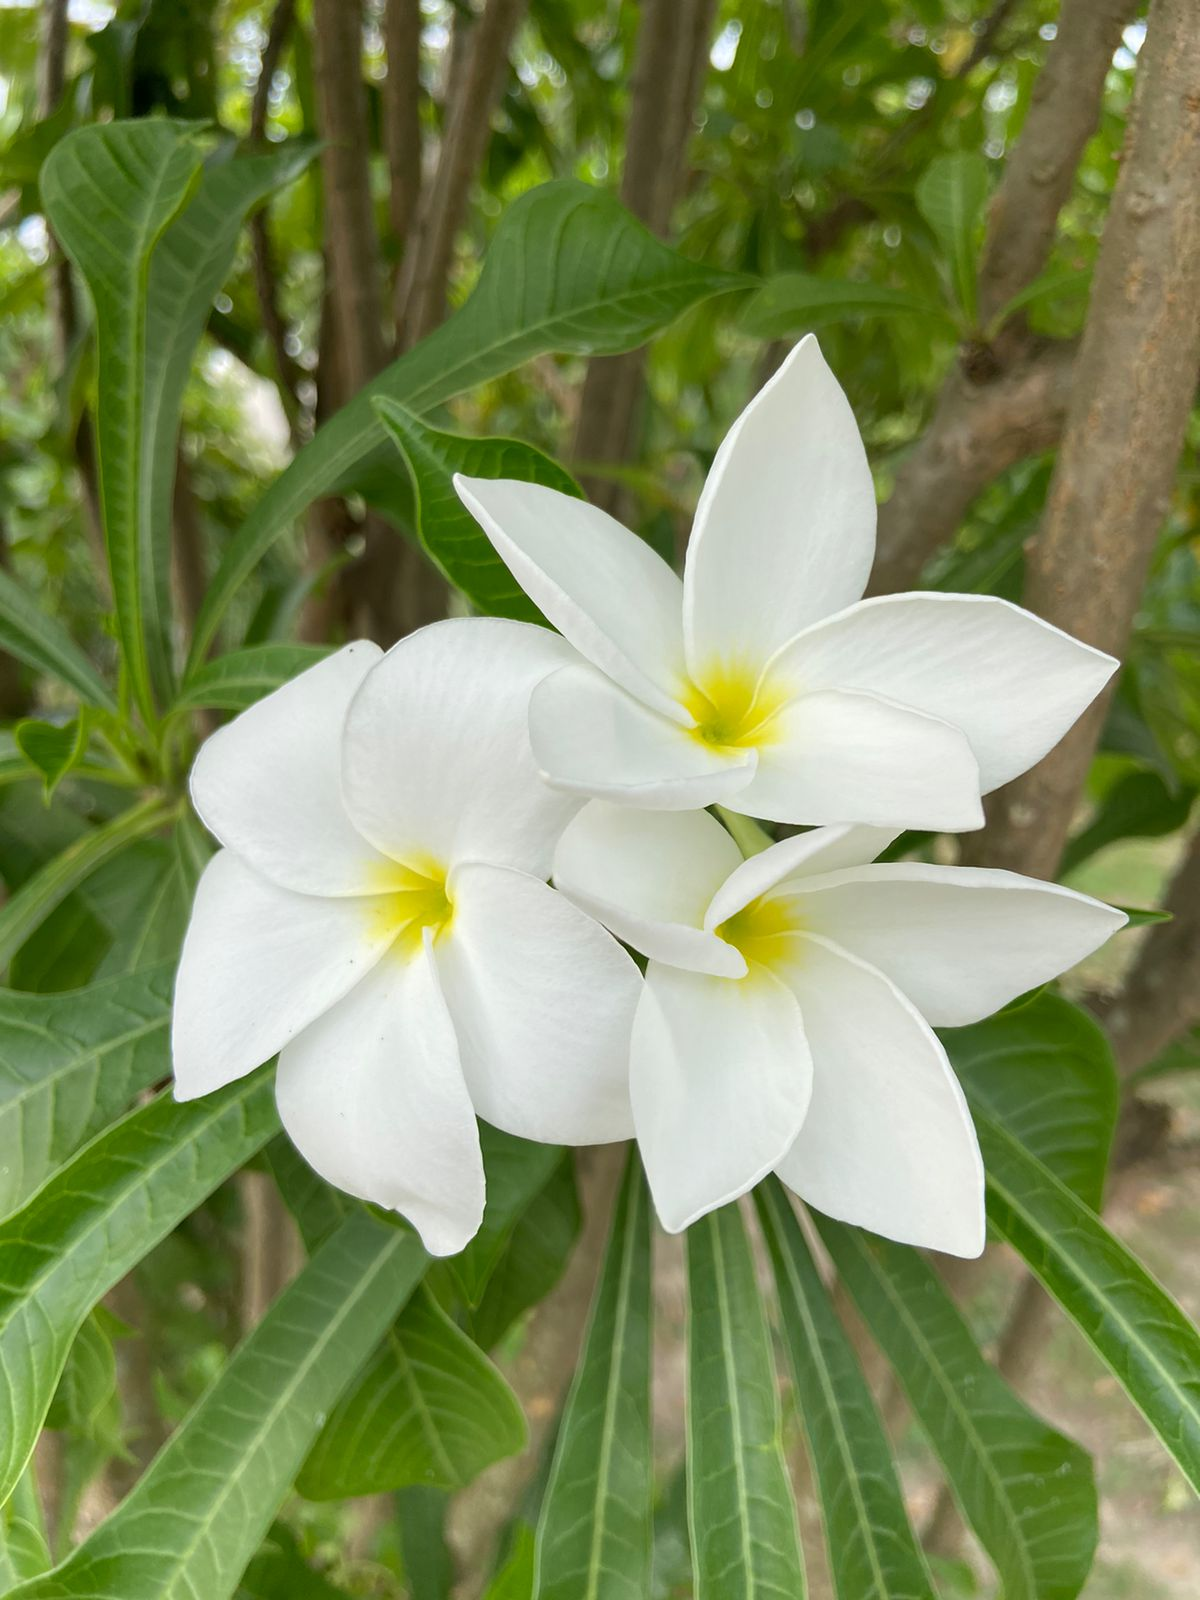
\includegraphics[scale=0.13]{images/pp.jpg}
\end{center}
\textbf{Scientific name:} Plumeria pudica\newline
\textbf{Common name:} Nag Champa\newline
\textbf{Family:} Apocynaceae\newline
\textbf{Location:} Near Visitor's hostel\newline
\textbf{Flower:} The flowers are bisexual and actinomorphic, and hypogynous. Plumeria pudica produces flowers in terminal clusters called panicles. These panicles consist of multiple individual flowers arranged in a branched or corymb-like structure. The flowers of Plumeria pudica are relatively small compared to other Plumeria species, measuring around 4-6 cm (1.5-2.5 inches) in diameter. They have a distinct shape and structure.\newline
\textbf{Pollination:} These flowers are hermaphrodidtic and self-pollination is the main form of pollination. Cross-pollination by insects also occurs.

\text{ }\newline
\textbf{Calyx:} The calyx has 5 unfused, greenish sepals.\newline
\textbf{Corolla:} The corolla has 5 white (with yellow center) petals that are fused forming a tube with the lobes overlapping to one side forming a pinwheel shape.\newline
\textbf{Androecium:} There are 5 stamens fused to the corolla tube.\newline
\textbf{Gynoecium:} The gynoecium is syncarpous, with a \textbf{superior ovary}, 2 carpels, and 2 locules. The style is solitary and terminal; the stigma is solitary, 2-lobed, or decurrent. Placentation is parietal with placentae sometimes protruding and branched, rarely axile or free-central; ovules are anatropous, unitegmic, numerous.
\section{Hibiscus rosa-sinensis}
\begin{center}
    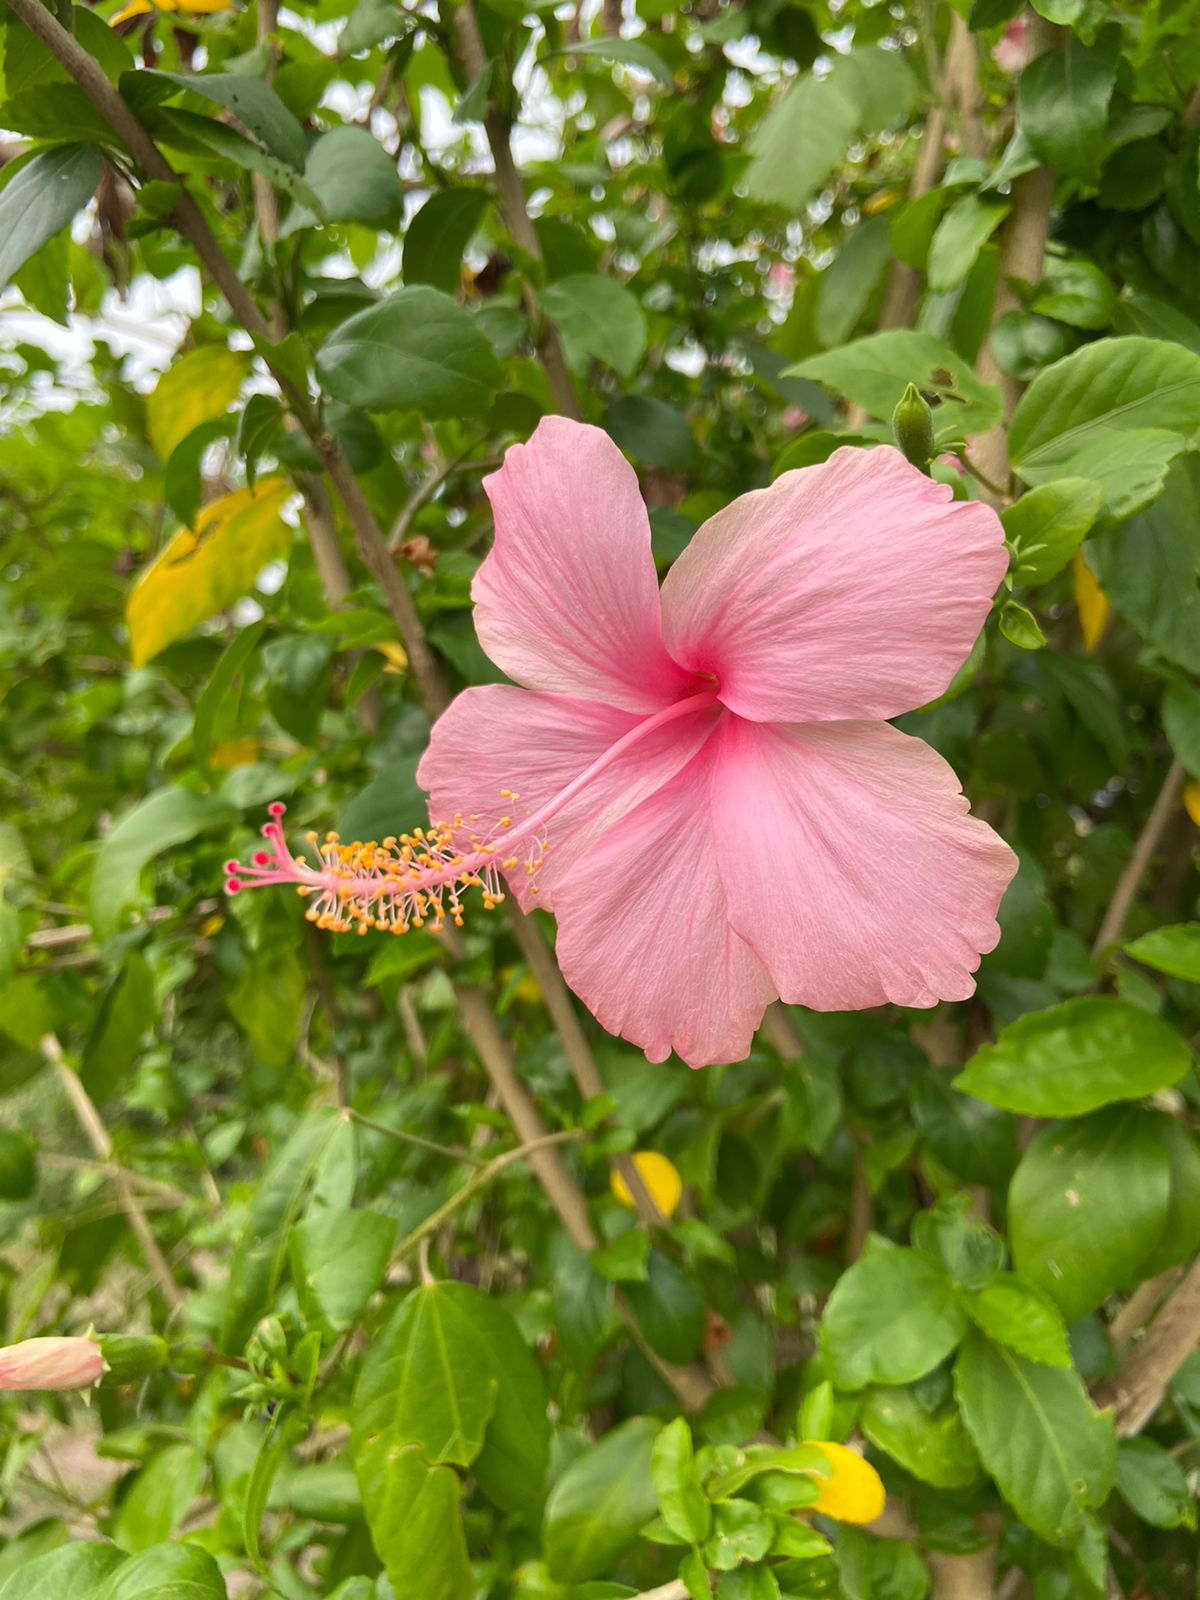
\includegraphics[scale=0.13]{images/shoe.jpg}
\end{center}
\textbf{Scientific name:} Hibiscus rosa-sinensis\newline
\textbf{Common name:} Chinese hibiscus\newline
\textbf{Family:} Malvaceae\newline
\textbf{Location:} Near Visitor's hostel\newline
\textbf{Flower:} Bisexual flower. Hibiscus rosa-sinensis produces solitary flowers, which means that each flower arises individually rather than in clusters. However, multiple flowers can be present on the plant simultaneously. The flowers of Hibiscus rosa-sinensis are large and eye-catching, typically measuring around 10-15 cm (4-6 inches) in diameter. They have a wide range of shapes, including single, double, and semi-double forms. \newline
\textbf{Pollination:} Pollination is primarily entomophilous i.e., by insects.   We observed a honeybee suck nectar from the photographed hibiscus flower.

\text{ }\newline
\textbf{Calyx: }Sepals 5, green, gamosepalous showing valvate aestivation and odd sepal is posterior in position.\newline
\textbf{Corolla:} The flowers have five large, overlapping petals that are broad and flat. The petals are typically broadest towards their outer edges and gradually taper towards the base. They may be rounded, obovate, or even lobed. Hibiscus rosa-sinensis flowers have a relatively long tubular structure called the corolla tube, which is located at the base of the petals. \newline
\textbf{Androecium:} Inside the corolla tube, there are numerous stamens, which are the male reproductive structures. Each stamen consists of a filament and an anther. The filaments are slender and elongated, while the anthers contain the pollen grains.\newline
\textbf{Gynoecium:} The flower of Hibiscus is composed of five carpels which are fused. The gynoecium in Hibiscus is multicarpellary and syncarpous.\newline

\textbf{\textit{Flower formula:}}
\begin{center}
    
\includegraphics{images/Screenshot 2023-06-21 235437.png}
\end{center}
\section{Duranta erecta}
\begin{center}
    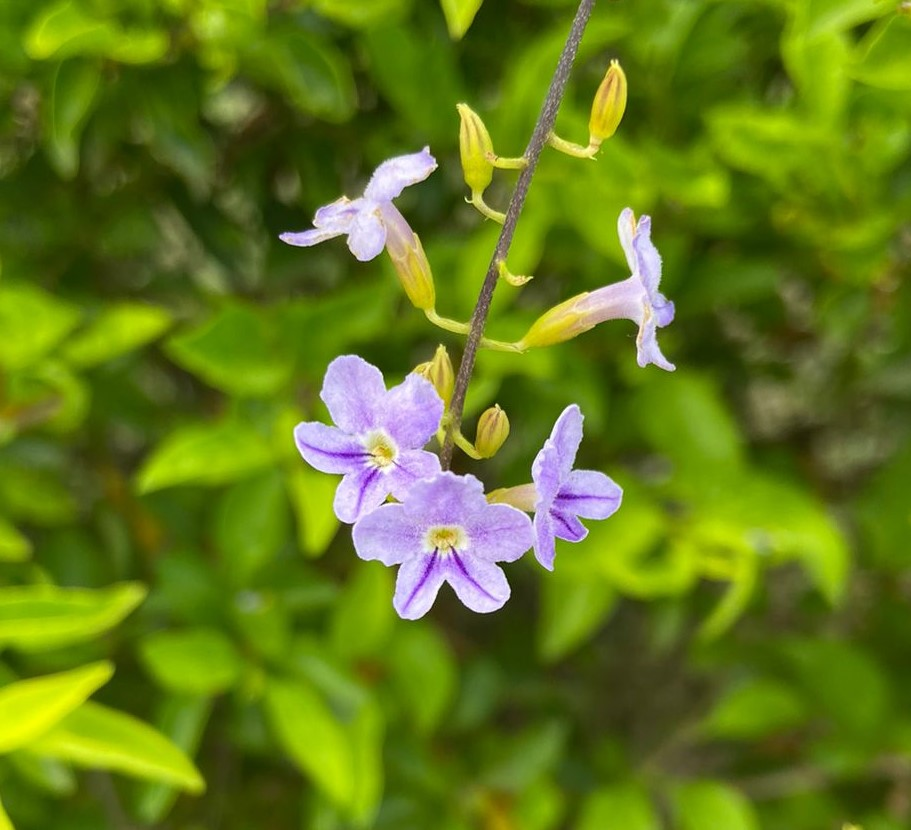
\includegraphics[scale=0.22]{images/blpr.jpg}
\end{center}
\textbf{Scientific name:} Duranta erecta\newline
\textbf{Common name:} Golden dewdrops\newline
\textbf{Family:}  Verbenaceae\newline
\textbf{Location:} Near NSCB mess\newline
\textbf{Flower:}Duranta species flowers are bisexual, i.e., with functional male (androecium) and female (gynoecium), including stamens, carpels and ovary. Duranta erecta produces small, tubular flowers that are arranged in loose, drooping clusters known as panicles. These panicles can vary in length and density, depending on the cultivar and growth conditions. \newline
\textbf{Pollination:} Pollination is entomophilous i.e., by insects.  
\newline
\textbf{}\newline
\textbf{Calyx:} Tubular or subhypocrateriform 5 toothed with acute teeth, sparsely pubescent and light green colored.\newline
\textbf{Corolla:} Corolla hypocrateriform, unequal 5 lobed, blue, purple and yellowish purple, apex truncate, Corolla tube sparsely hairy on the throat, lateral lobes straight or curved.\newline
\textbf{Androecium:} 4 stamen, didynamous, inserted in the corolla tube, filaments filiform, 2-2.5 mm long, hairy, green colored, anthers creamish, oblong.\newline
\textbf{Gynoecium:} Ovary globose about 1 mm long, style slender about half the length of the corolla tube, glabrous, Stigma capitates, shortly 4 lobed. Fruit drupe globose about 0.75-1 cm in diameter, shining yellow.
\end{document}

